\chapter{Introduction}

Ce projet consiste a développer une simulation qui permet la gestion d'un carrefour entre deux routes à sens unique avec deux feux de signalisations. L'objectif est de permettre la gestion du système en utilisant des réseau de Petri qui interagit avec le monde réel au moyen d'événement extérieur et d'action déclenché par les places du réseau.

Dans le cadre du projet deux phases ont été réalisées, la première phase consistait à développer le système sans utiliser de timer gérer par réseau de Petri, à la place une simple attente était effectué entre le changement des états des feux. Ce rapport décrit la deuxième phase qui consiste à avoir deux réseau de Petri fonctionnant en parallèle, un pour la gestion du carrefour, et le deuxième pour la gestion d'un timer.

La figure~\ref{fig:gui} montre une vue de l'interface graphique de la simulation. Sur le GUI sont représenté les éléments du système, les voitures évoluant sur la route, les feux de signalisation ainsi que le détecteur de véhicule avant le carrefour (zone en jaune claire quand il n'y a pas de véhicule, et jaune foncé lorsque des véhicules sont détectés). Enfin l'interface dispose d'un bouton (en haut à gauche), qui permet de tuer les Threads de génération de véhicule, ce qui termine la simulation.

\begin{figure}[htb]
\centering 
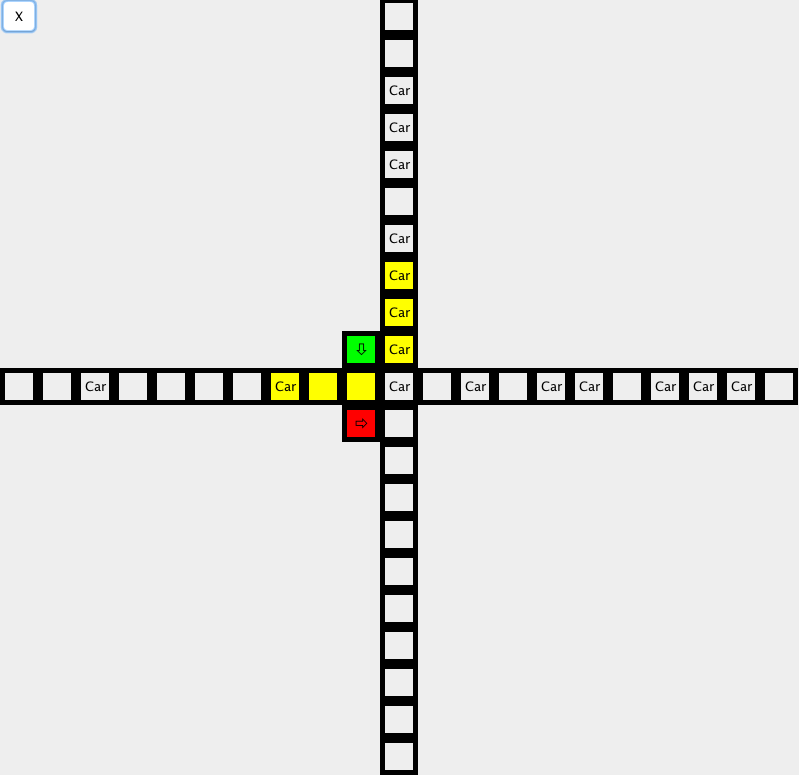
\includegraphics[width=0.8\columnwidth]{gui}
\caption[Interface graphique de l'application]{Interface graphique de l'application}
\label{fig:gui}
\end{figure}